% ==================== PROGETTAZIONE DELL'APPLICATIVO ============================

\newpage

\enlargethispage{1\linewidth}

\section{Progettazione dell'Applicativo}

\textsf{\small L'applicativo per poter interagire con la base di dati è stato sviluppato in \textbf{JavaFX}, usufruendo dello strumento di creazione di interfaccie grafiche \textbf{Scene Builder}. }\\

\textsf{\small Per quanto riguarda l'immagazzinamento del database è stato eseguito in locale con \textbf{MySQL}.}\\

\begin{figure}[ht] 
	\centering
	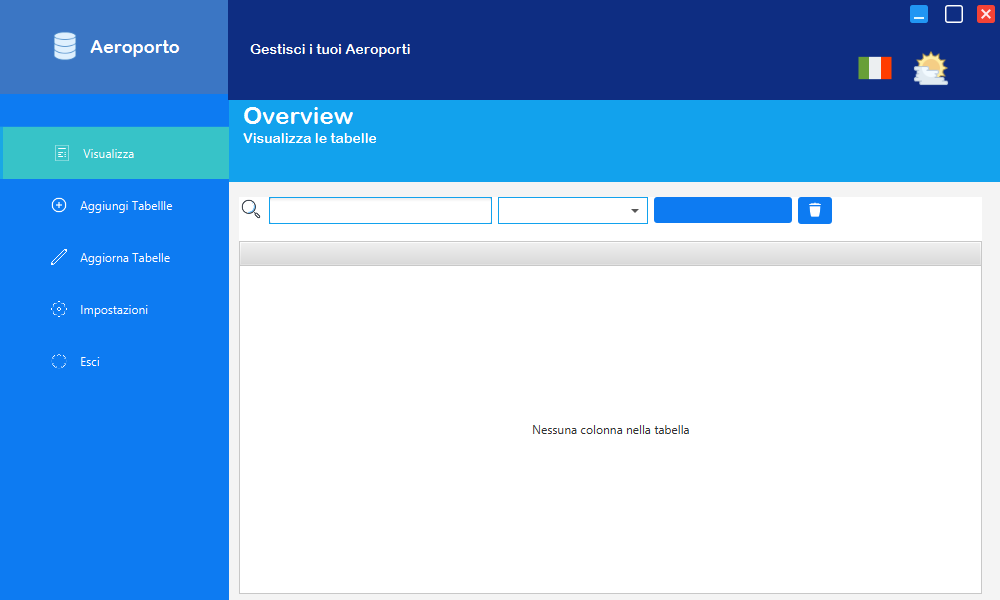
\includegraphics[width=1\textwidth, height=1\textheight, keepaspectratio]{./img/Applicativo/homepage.png}
	\caption{Homepage dell'Applicativo.}
	\label{fig:homepage}
\end{figure}

\textsf{\small Esso presenta svariate funzionalità necessarie per l'interazione col database e opzionali: } 

\begin{itemize}
	\item \textsf{\small Visualizzazione delle tabelle.}
	\item \textsf{\small Aggiunta di righe nelle tabelle.}
	\item \textsf{\small Modifica dei dati delle righe.}
	\item \textsf{\small Rimozione di specifiche righe selezionate dall'utente.}
	\item \textsf{\small Messaggi per notificare l'utente sull'esecuzione o meno dell'operazione scelta.}
	\item \textsf{\small Barra di ricerca per poter trovare gli elementi di una tabella più facilmente.}
	\item \textsf{\small Possibilità di modificare la lingua in Inglese o in Italiano.}
	\item \textsf{\small Possibilità di modificare il tema del software in chiaro o scuro.}
	\item \textsf{\small Possibilità di salvare la lingua e il tema scelti in un file di impostazioni sicuro criptato tramite lo \emph{Advanced Encryption Standard} (\textbf{AES}).}
	\item \textsf{\small Possibilità di resettare le impostazioni di default.}
	%\item \textsf{\small }
\end{itemize}

% ========================== OVERVIEW ==========================================

\newpage

\enlargethispage{1\linewidth}

\subsection{Overview | Visualizza}

\textsf{\small Questa schermata permette all'utente in base ad una scelta dal \emph{combo box} di poter selezionare la tabella da visionare. (L'immagine \ref{fig:maximize} fa uso del tema scuro e della lingua inglese)}\\

\begin{figure}[ht]
	\begin{subfigure}{.6\textwidth}
		\centering
		%\flushleft
		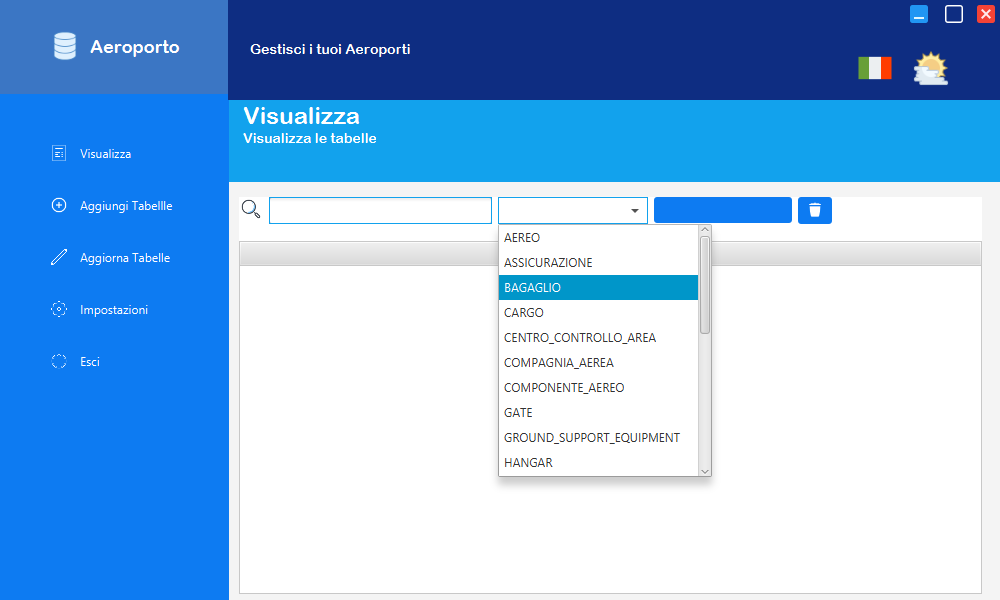
\includegraphics[width=1\linewidth]{./img/Applicativo/homepage_overview_table_selection.png}
		\caption{Selezione tabella}
		\label{fig:overview1}
	\end{subfigure}%
	\begin{subfigure}{.6\textwidth}
		\centering
		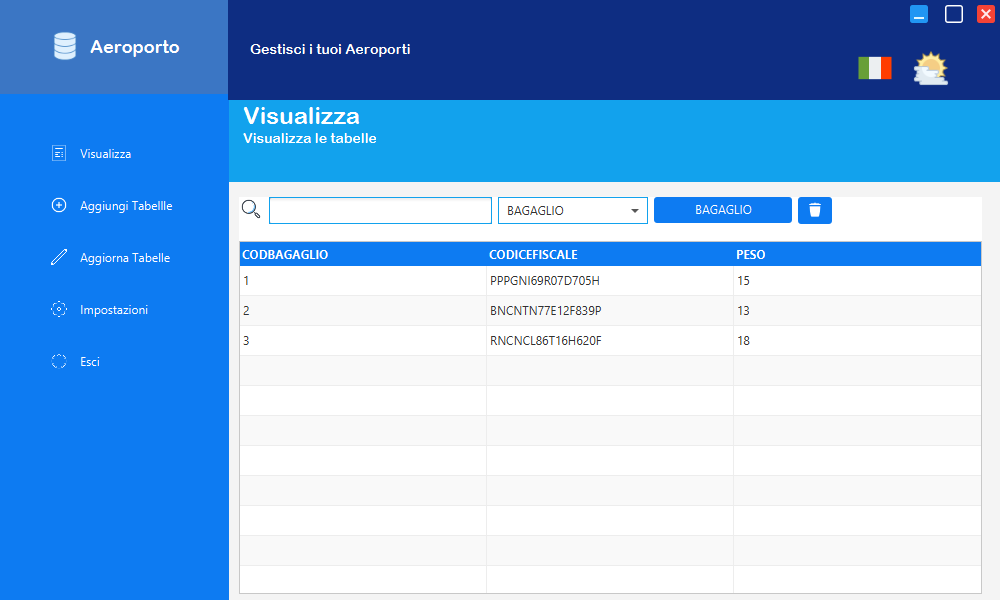
\includegraphics[width=1\linewidth]{./img/Applicativo/homepage_overview_table_selection2.png}
		\caption{Visualizzazione tabella selezionata}
		\label{fig:overview2}
	\end{subfigure}
	%\caption{a}
	\label{fig:overviews}
\end{figure}


\begin{figure}[H] 
\centering
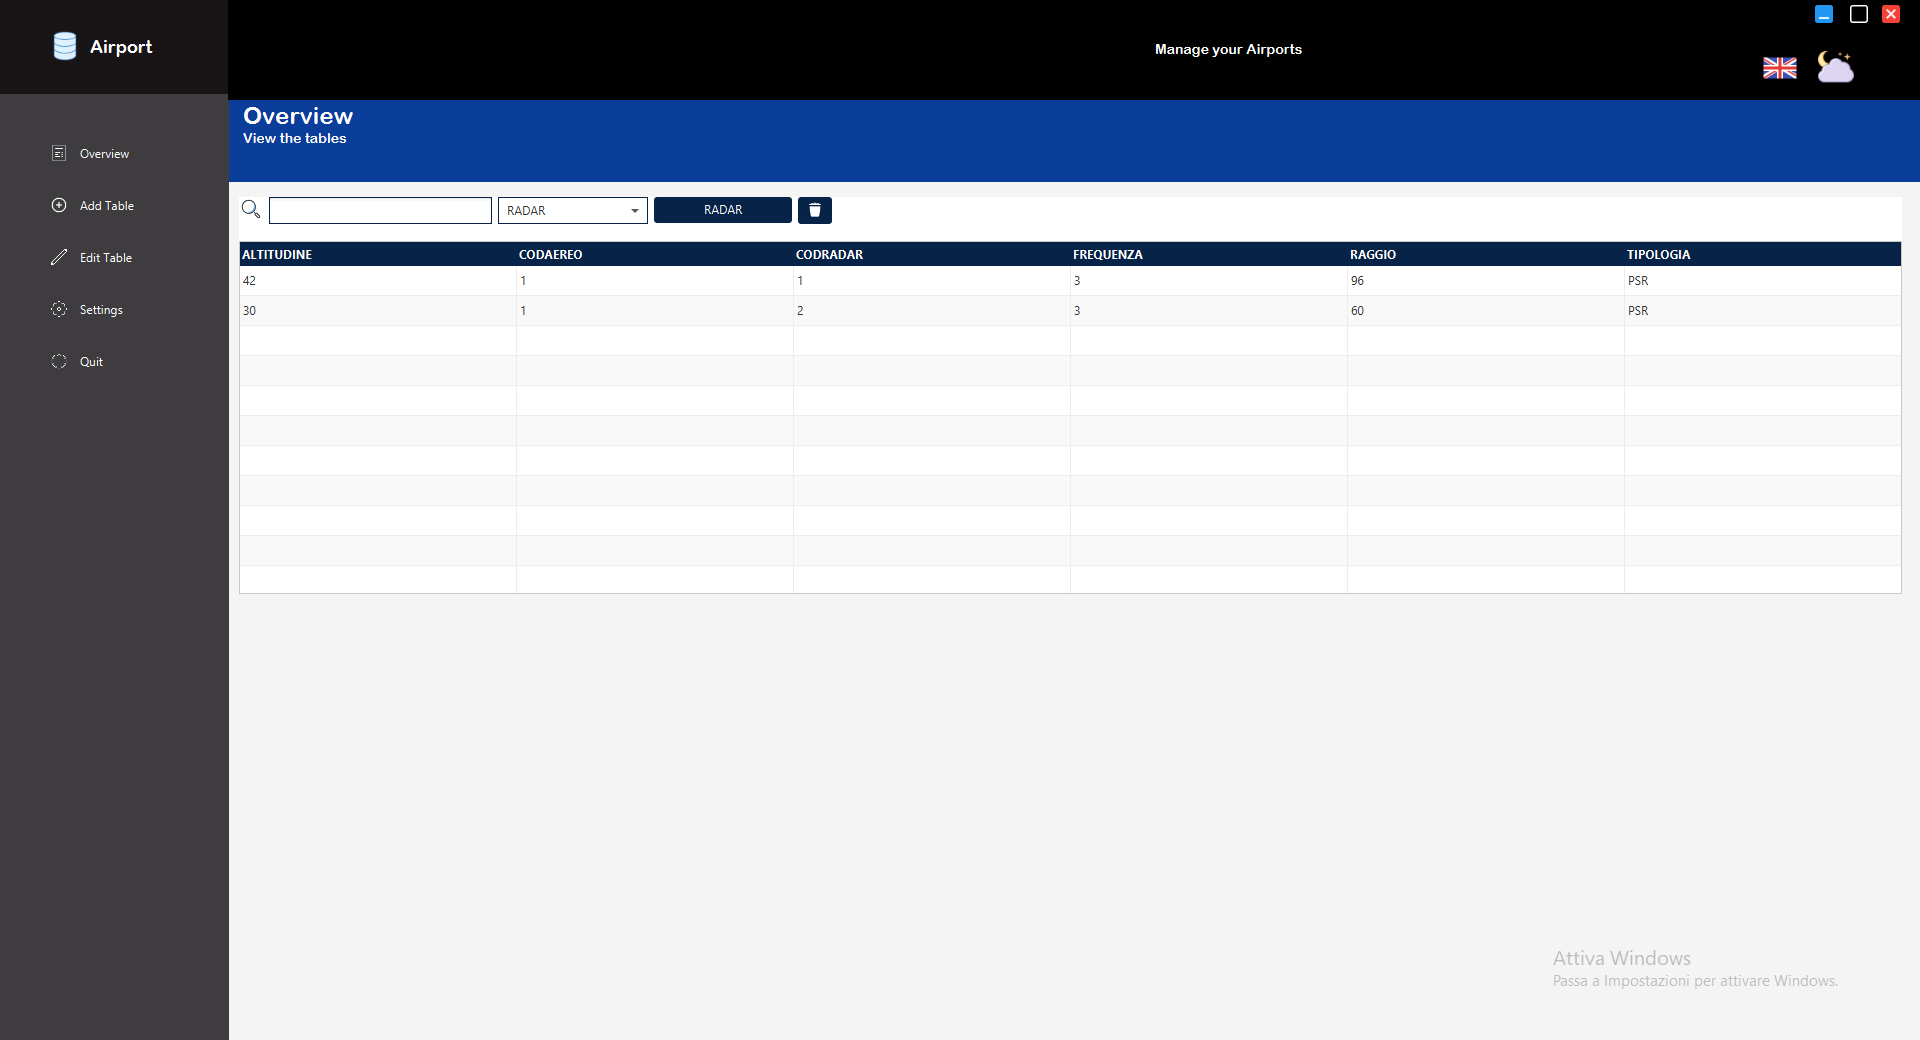
\includegraphics[width=1\textwidth, height=1\textheight, keepaspectratio]{./img/Applicativo/maximize.png}
\caption{Homepage dell'Applicativo schermata massimizzata.}
\label{fig:maximize}
\end{figure}


\textsf{\small Inoltre son presenti due ulteriori funzionalità: quella di poter ricercare elementi dalla barra di ricerca e quella di poter eliminare una determinata riga selezionata di una tabella.}\\

% ========================== SEARCH BAR =======================================

\pagebreak

%\enlargethispage{1\linewidth}

\subsubsection{Search Bar | Barra di Ricerca}

\textsf{\small La barra di ricerca trova tutti gli elementi scritti in essa. Se una data informazione si trova in più righe allora mostra tutte le righe, altrimenti solo una oppure nessuna se il dato cercato non è presente nella tabella in questione.}

\begin{figure}[H] 
	\centering
	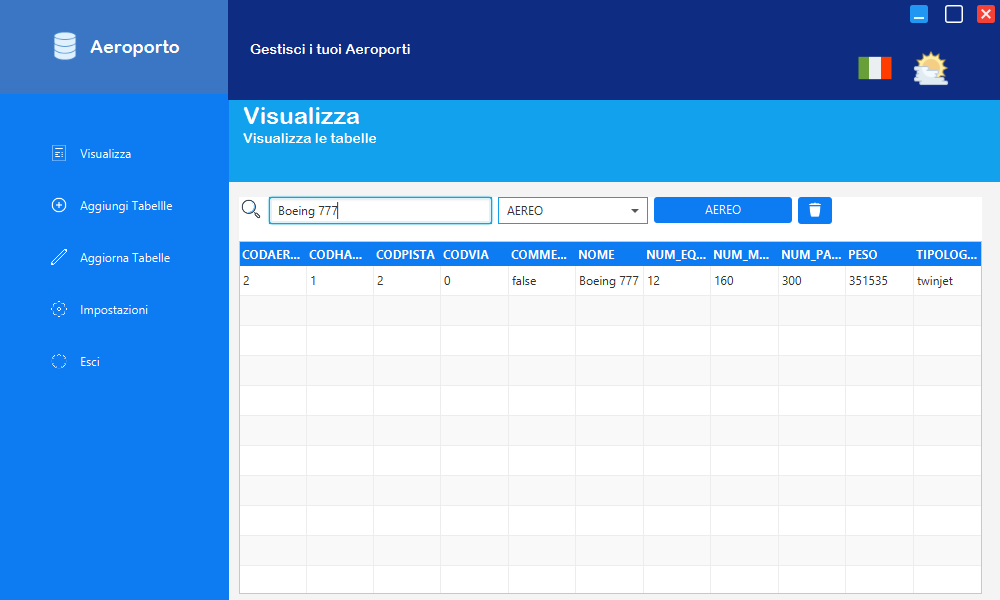
\includegraphics[width=1\textwidth, height=1\textheight, keepaspectratio]{./img/Applicativo/search_bar2.png}
	\caption{Ricerca di uno specifico aereo.}
	\label{fig:search_bar2}
\end{figure}

\begin{figure}[H]
	\begin{subfigure}{.6\textwidth}
		\centering
		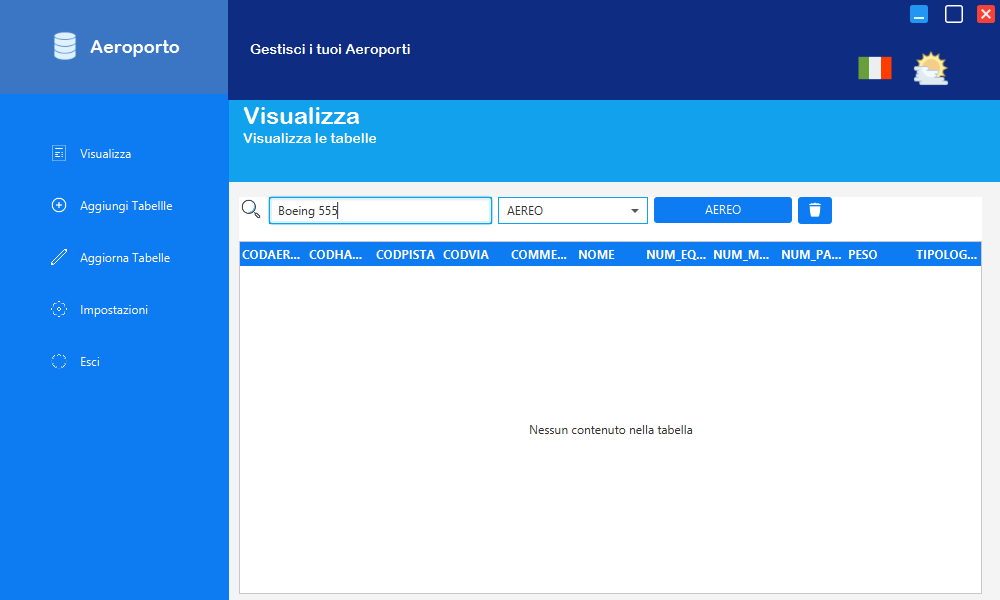
\includegraphics[width=1\linewidth]{./img/Applicativo/search_bar3.png}
		\caption{Ricerca non trovata perchè elemento non presente.}
		\label{fig:search_bar3}
	\end{subfigure}%
	\begin{subfigure}{.6\textwidth}
		\centering
		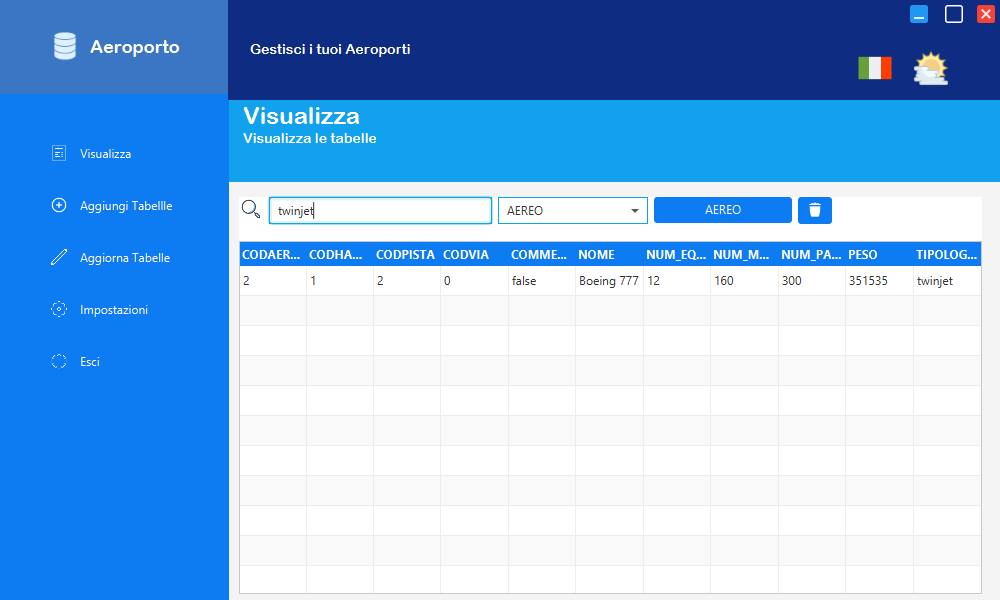
\includegraphics[width=1\linewidth]{./img/Applicativo/search_bar4.png}
		\caption{Ricerca trovata}
		\label{fig:search_bar4}
	\end{subfigure}
	%\caption{a}
	\label{fig:search_bars}
\end{figure}

\begin{figure}[H]
	\begin{subfigure}{.6\textwidth}
		\centering
		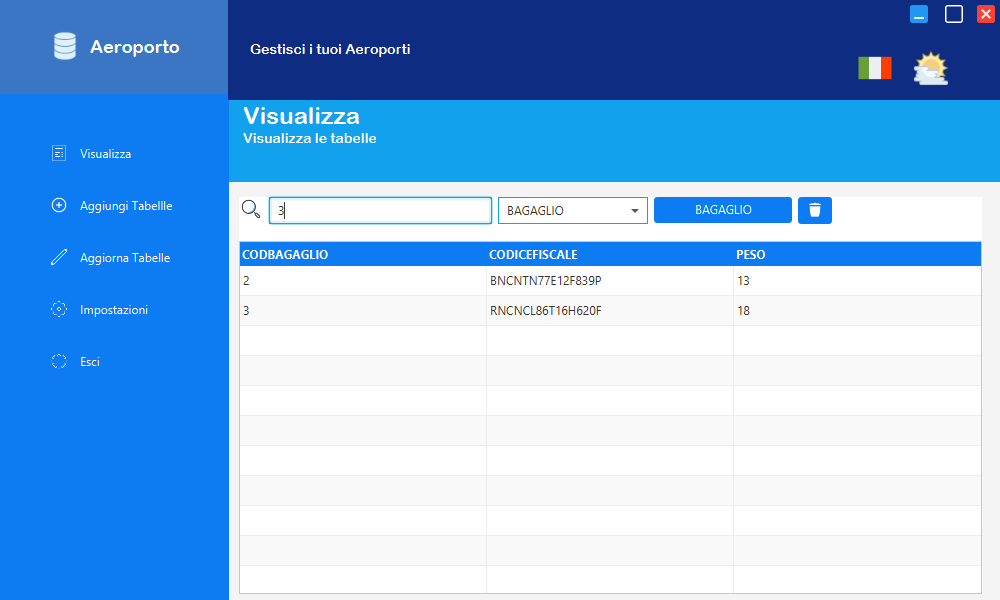
\includegraphics[width=1\linewidth]{./img/Applicativo/search_bar7.png}
		\caption{Trovati due elementi con quelle specifiche}
		\label{fig:search_bar7}
	\end{subfigure}%
	\begin{subfigure}{.6\textwidth}
		\centering
		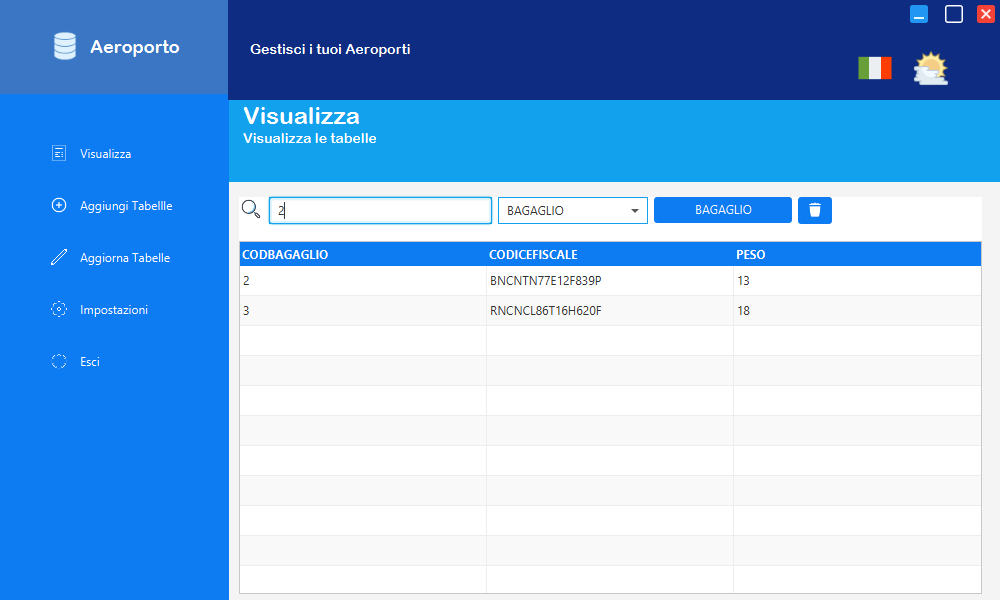
\includegraphics[width=1\linewidth]{./img/Applicativo/search_bar8.png}
		\caption{Trovati due elementi con quelle specifiche}
		\label{fig:search_bar8}
	\end{subfigure}
	%\caption{a}
	\label{fig:search_bars2}
\end{figure}

% ========================== DELETE ===========================================

%\pagebreak

\enlargethispage{1\linewidth}

\subsubsection{Delete | Rimozione}

\textsf{\small Tramite l'interruttore \emph{Cancella}, quello con l'icona del cestino, una volta selezionata la riga e aver confermato l' \emph{Alert} che chiede all'utente se è sicuro di voler procedere, l'elemento verrà cancellato.}

\begin{figure}[H] 
	\centering
	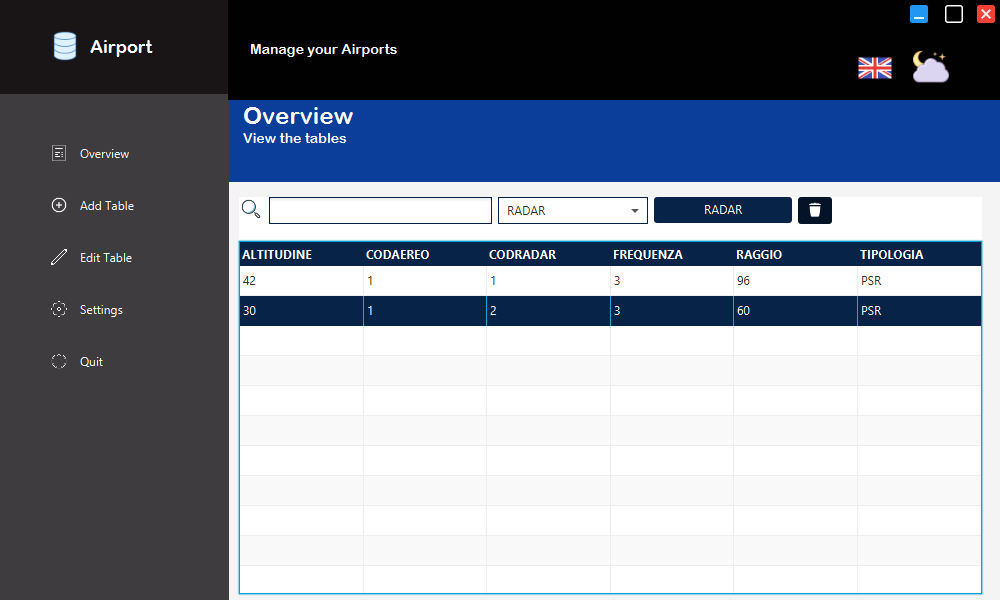
\includegraphics[width=1\textwidth, height=1\textheight, keepaspectratio]{./img/Applicativo/delete_data.png}
	\caption{Cancellazione della suddetta riga di dati.}
	\label{fig:delete_data}
\end{figure}

\pagebreak

\begin{figure}[H] 
	\centering
	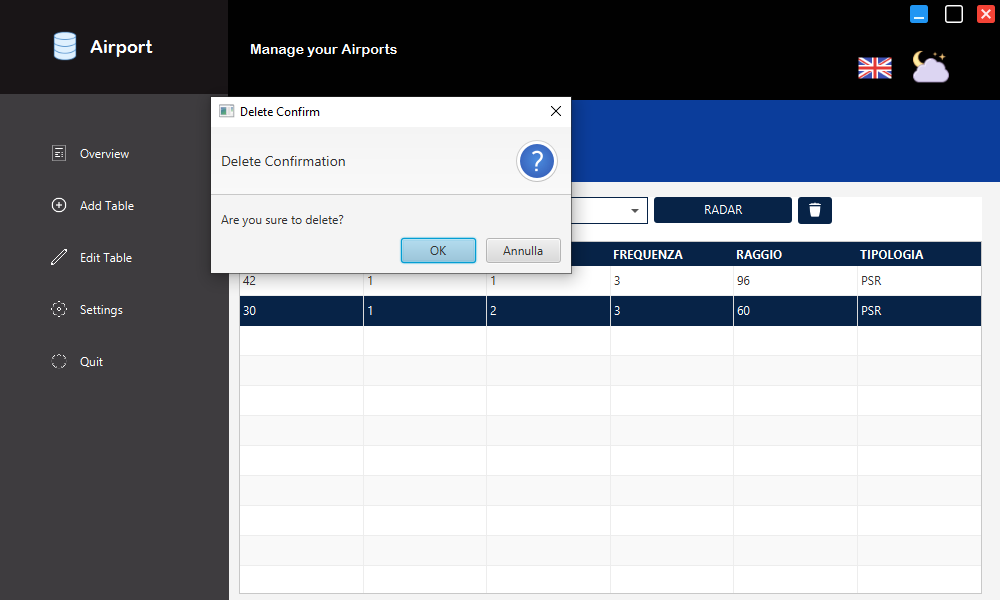
\includegraphics[width=1\textwidth, height=1\textheight, keepaspectratio]{./img/Applicativo/delete_alert_confirmation.png}
	\caption{Conferma cancellazione Alert.}
	\label{fig:delete_alert_confirmation}
\end{figure}

%\pagebreak

\begin{figure}[H]
	\begin{subfigure}{.6\textwidth}
		\centering
		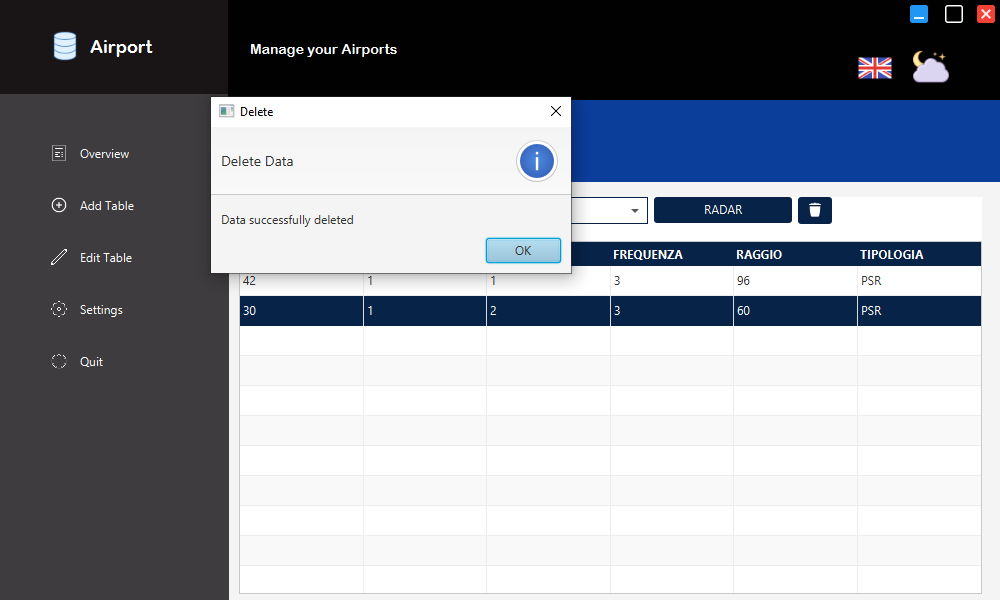
\includegraphics[width=1\linewidth]{./img/Applicativo/delete_data_success.png}
		\caption{Alert eliminazione con successo}
		\label{fig:delete_alert_success}
	\end{subfigure}%
	\begin{subfigure}{.6\textwidth}
		\centering
		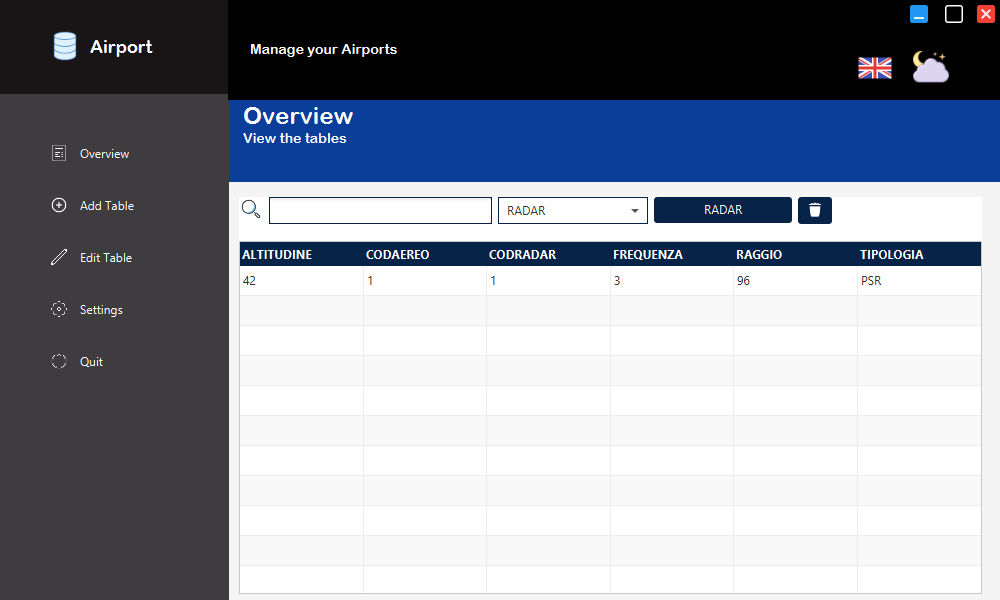
\includegraphics[width=1\linewidth]{./img/Applicativo/delete_data_aftermath.png}
		\caption{Visualizzazione della tabella dopo la cancellazione}
		\label{fig:delete_data_aftermath}
	\end{subfigure}
	%\caption{a}
	\label{fig:overviews2}
\end{figure}

% ========================== ADD TAB ==========================================

\newpage

\subsection{Add | Aggiungi}

\textsf{\small La scheda Aggiungi permette all'utente, una volta selezionata una tabella, attraverso i campi di testo di aggiungere una riga di dati alla tabella in questione.}\\

\begin{figure}[H] 
	\centering
	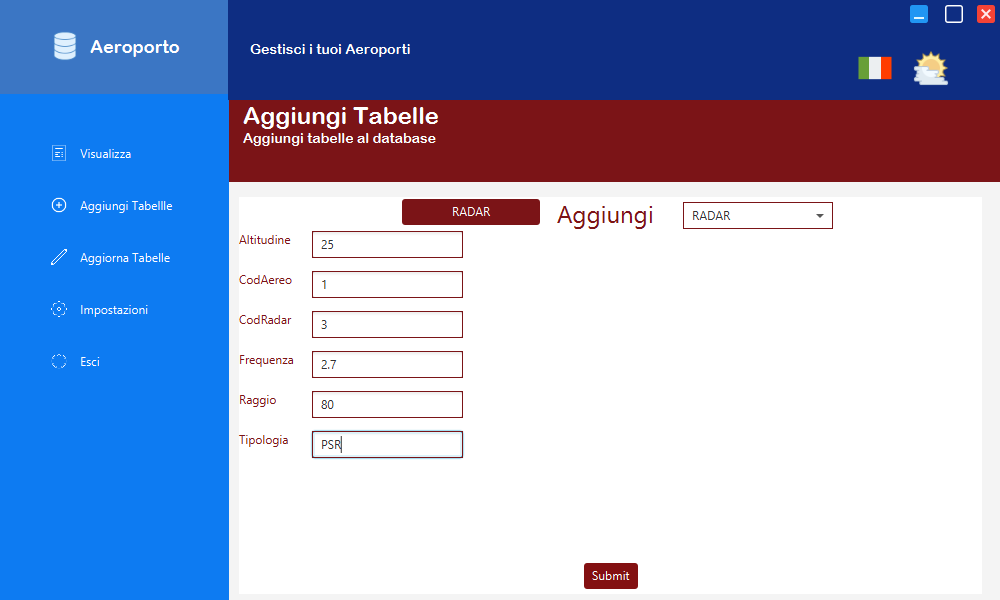
\includegraphics[width=1\textwidth, height=1\textheight, keepaspectratio]{./img/Applicativo/add_table.png}
	\caption{Aggiunta riga con i text fields.}
	\label{fig:add_table}
\end{figure}

\textsf{\small Dopo che l'utente avrà riempito i boxes e avrà premuto il pulsante \emph{Submit} l'operazione verrà eseguita e un \emph{Alert} lo notificherà se è andata a successo o se si sono verificati degli errori. (Nell'immagine \ref{fig:add_alert_error} viene mostrata la schermata con l'utilizzo del tema scuro) }\\

\begin{figure}[ht]
	\begin{subfigure}{.6\textwidth}
		\centering
		%\flushleft
		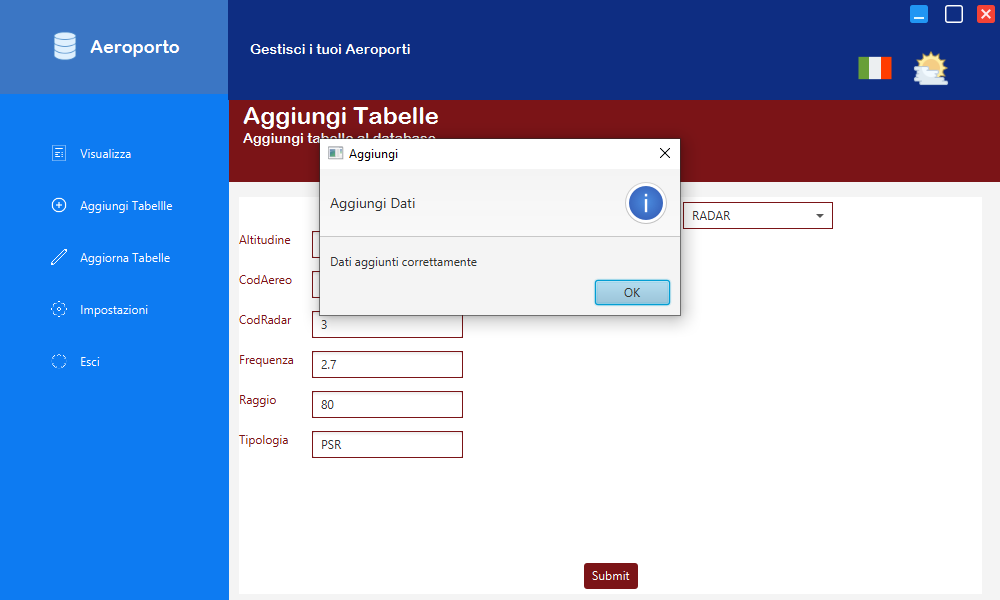
\includegraphics[width=1\linewidth]{./img/Applicativo/add_table_alert_success.png}
		\caption{Alert operazione eseguita con successo}
		\label{fig:add_alert_success}
	\end{subfigure}%
	\begin{subfigure}{.6\textwidth}
		\centering
		%\flushleft
		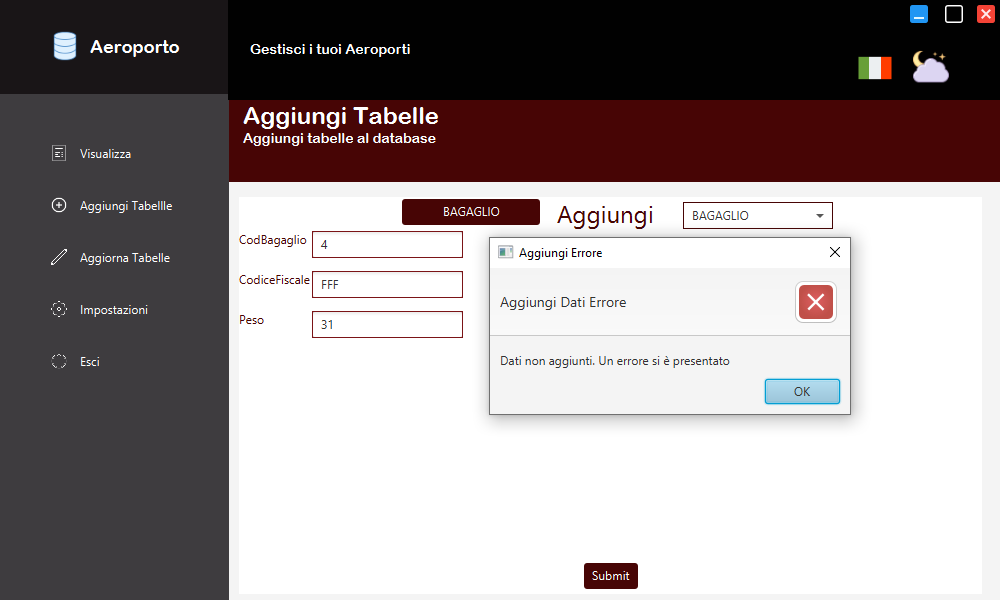
\includegraphics[width=1\linewidth]{./img/Applicativo/add_table_alert_error.png}
		\caption{Alert operazione non eseguita. Errori presenti}
		\label{fig:add_alert_error}
	\end{subfigure}
	%\caption{Add Tab Alerts}
	\label{fig:adds}
\end{figure}

% ========================== EDIT TAB ==========================================

\newpage

\enlargethispage{1\linewidth}

\subsection{Edit | Modifica}

\textsf{\small Tramite questa schermata, una volta scelta la tabella da modificare, dei campi di testo compariranno sulla sinistra.}\\

\begin{figure}[H] 
	\centering
	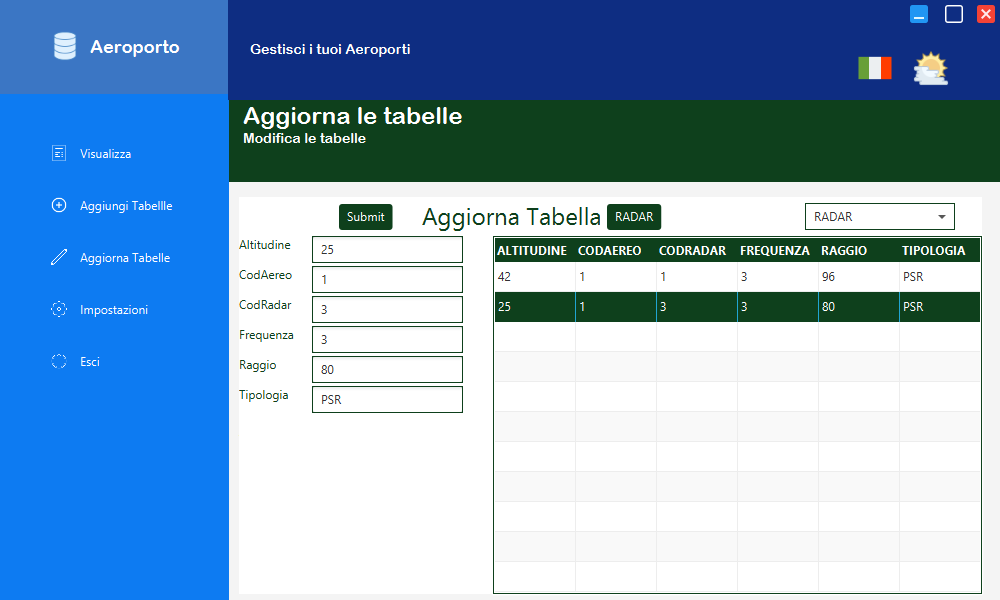
\includegraphics[width=1\textwidth, height=1\textheight, keepaspectratio]{./img/Applicativo/edit_table.png}
	\caption{Selezionata riga e dati automaticamente presentati nei text fields.}
	\label{fig:edit_table1}
\end{figure}

\textsf{\small Una volta selezionata la riga della tabella che si vuole editare i dati compariranno nei campi di testo e potranno essere modificati dall'utente.}\\

\begin{figure}[H] 
	\centering
	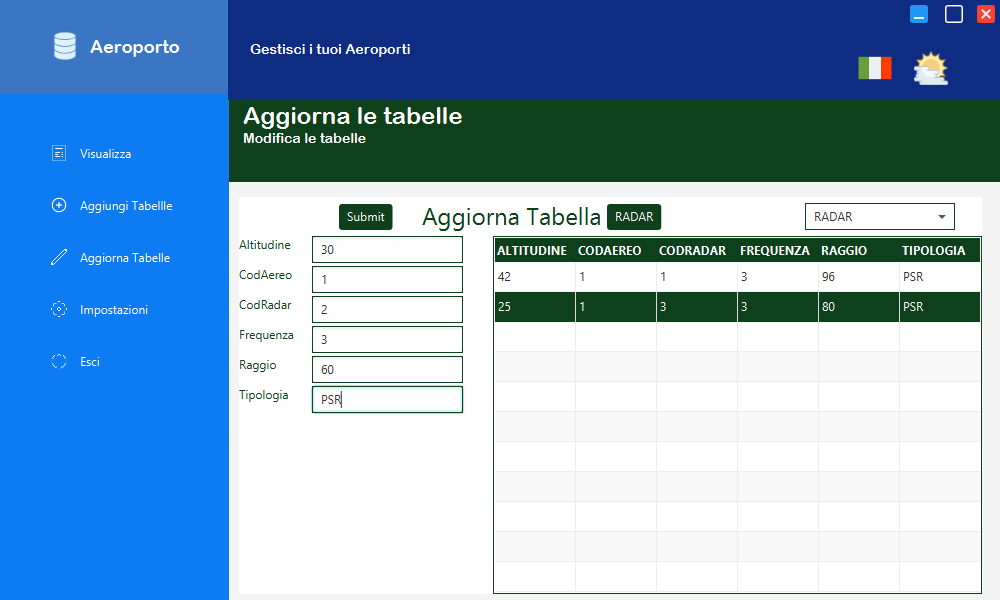
\includegraphics[width=1\textwidth, height=1\textheight, keepaspectratio]{./img/Applicativo/edit_table2.png}
	\caption{Modifica dei dati attraverso i text fields.}
	\label{fig:edit_table2}
\end{figure}

\pagebreak

\enlargethispage{1\linewidth}

\textsf{\small Come per la precedente operazione, una volta premuto \emph{Submit} un \emph{Alert} comparirà e avviserà l'utente. (Nell'immagine \ref{fig:edit_table_alert_error} è stata modificata la lingua in inglese e l'alert viene mostrato in quella lingua)}\\

\begin{figure}[H] 
	\centering
	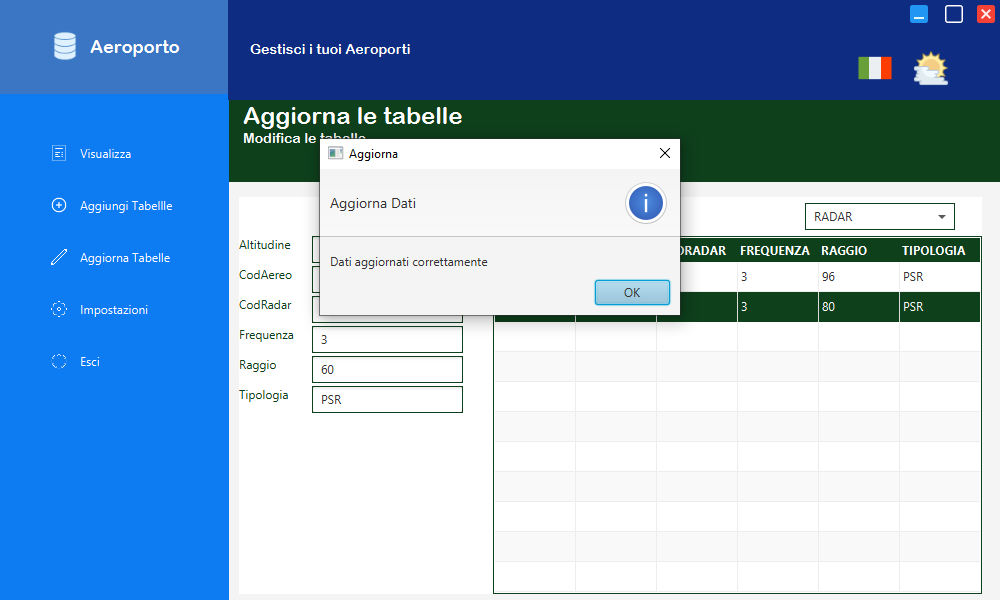
\includegraphics[width=1\textwidth, height=1\textheight, keepaspectratio]{./img/Applicativo/edit_table_alert.png}
	\caption{Alert operazione modifica eseguita con successo.}
	\label{fig:edit_table_alert_success}
\end{figure}

\begin{figure}[H] 
	\centering
	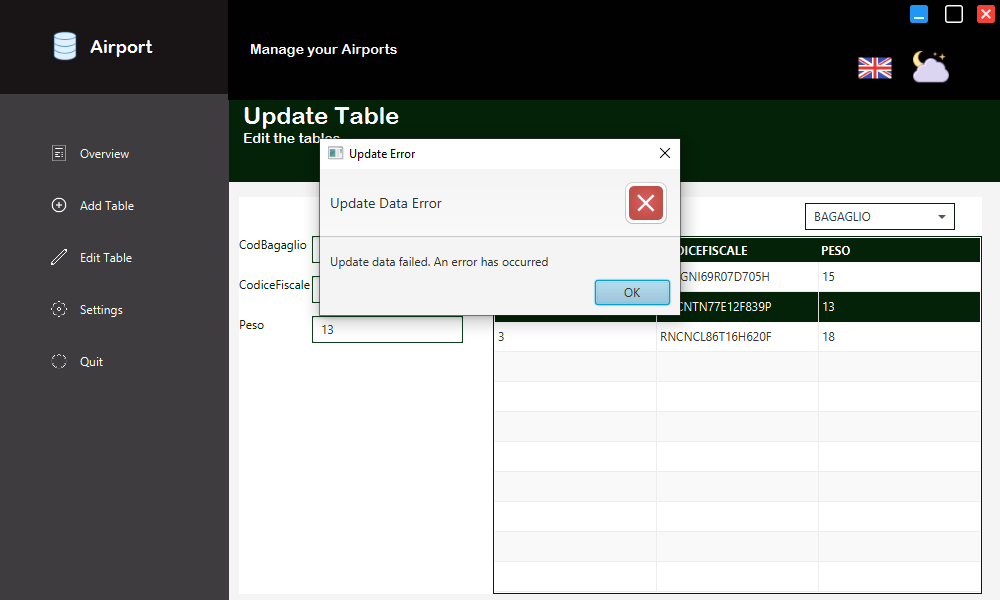
\includegraphics[width=1\textwidth, height=1\textheight, keepaspectratio]{./img/Applicativo/edit_table_alert_error.png}
	\caption{Alert operazione modifica eseguita con successo.}
	\label{fig:edit_table_alert_error}
\end{figure}

% ========================== SETTINGS TAB =====================================

\newpage

\enlargethispage{1\linewidth}

\subsection{Settings | Impostazioni}

\textsf{\small Questa è la pagina delle impostazioni, ce ne sono due possibili, questa sono la Lingua e il Tema del software.}

\begin{figure}[H] 
	\centering
	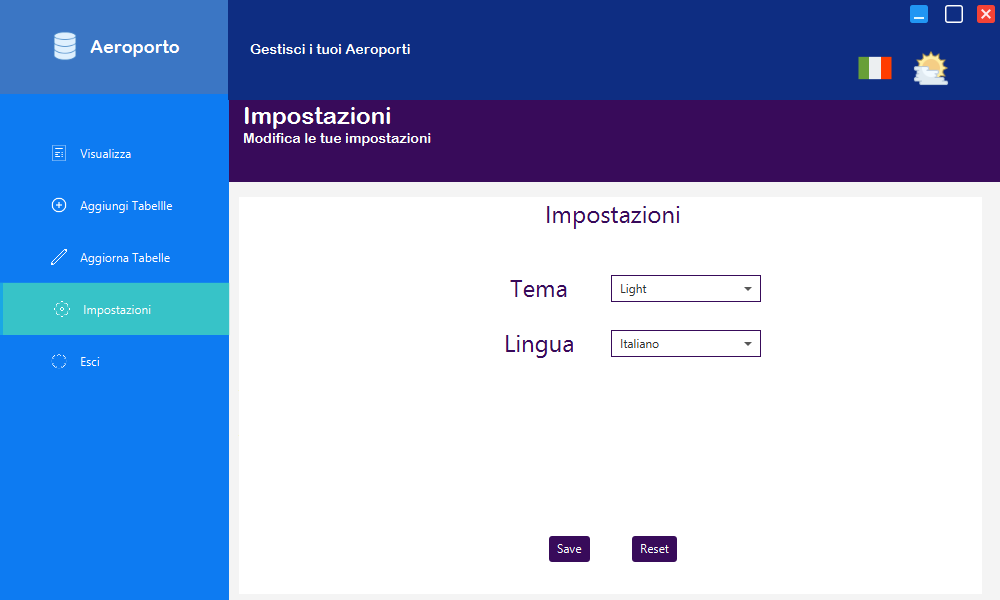
\includegraphics[width=1\textwidth, height=1\textheight, keepaspectratio]{./img/Applicativo/settings.png}
	\caption{Pannello delle Impostazioni.}
	\label{fig:settings1}
\end{figure}

\textsf{\small Queste possono essere modificate qui, nel pannello delle impostazioni oppure semplicemente cliccando le rispettive icone in alto a destra, in questo modo l'impostazione attuale verrà cambiata con l'altra possibile impostazione.}

\begin{figure}[H] 
	\centering
	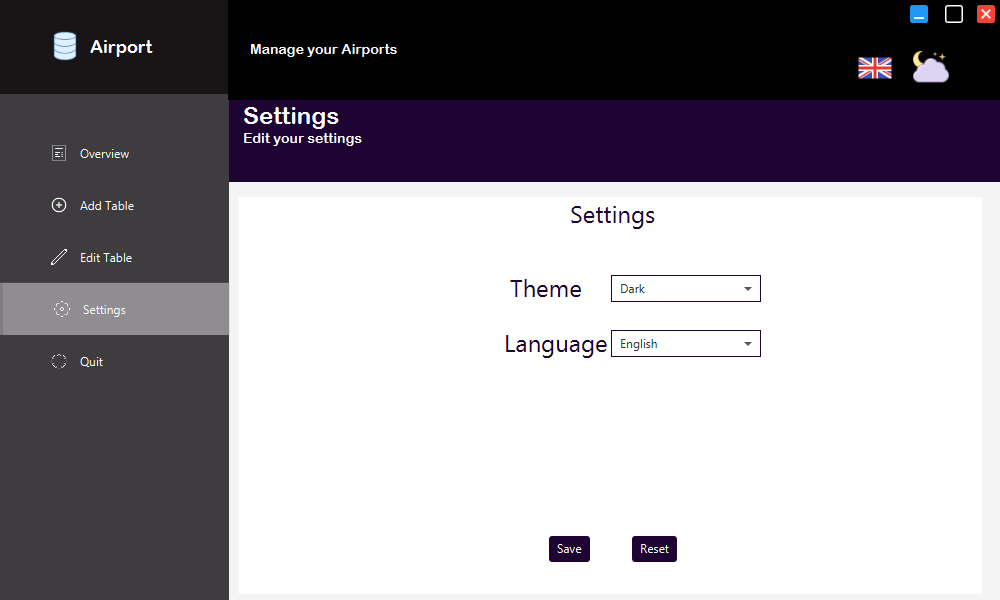
\includegraphics[width=1\textwidth, height=1\textheight, keepaspectratio]{./img/Applicativo/settings_change_language_and_theme.png}
	\caption{Impostazioni modificate e in tempo reale i cambiamenti vengono attuati.}
	\label{fig:settings2}
\end{figure}

% ========================== SAVE TAB =========================================

\pagebreak

\enlargethispage{1\linewidth}

\subsubsection{Save | Salvataggio}

\textsf{\small Attraverso il tasto \emph{Save} potranno essere salvate le impostazioni selezionate nei due combo box.}\\

\begin{figure}[H] 
	\centering
	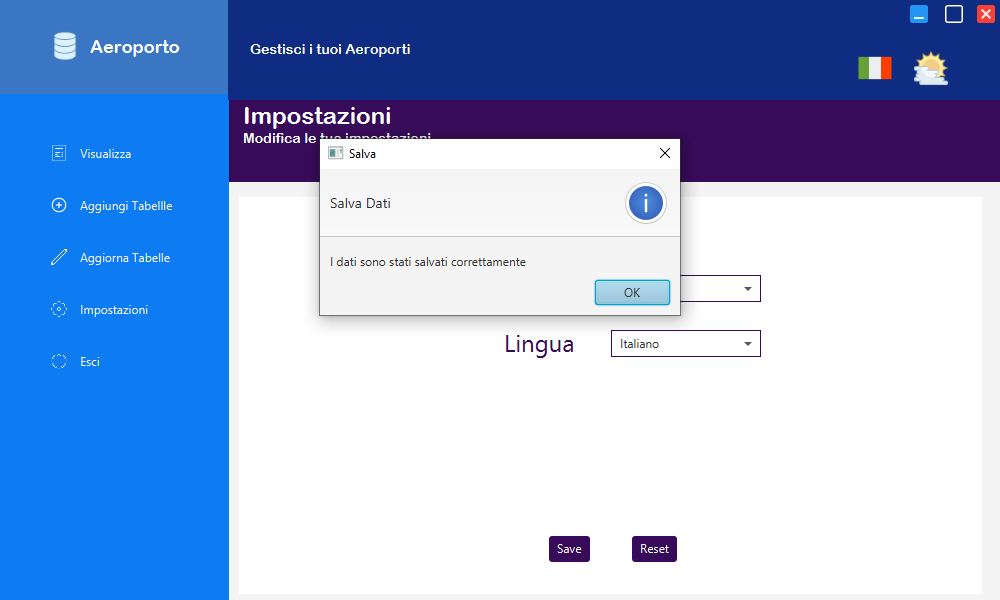
\includegraphics[width=1\textwidth, height=1\textheight, keepaspectratio]{./img/Applicativo/salvataggio.png}
	\caption{Salvataggio delle impostazioni e alert di conferma}
	\label{fig:save_alert_success}
\end{figure}

\textsf{\small Col pulsante \emph{Reset} si potrà resettare le impostazioni a quelle di default, ovvero Lingua : \emph{Inglese} e Tema : \emph{Chiaro}. Questo pulsante però, si limita a cambiare le impostazioni nei combo box e nelle icone, ma non a salvarle.}\\

\textsf{\small Queste impostazioni vengono salvate in un file JSON chiamato \emph{settings.dat} e criptato attraverso l' \emph{Advanced Encryption Standard} (\textbf{AES}).}\\

\begin{figure}[H] 
	\centering
	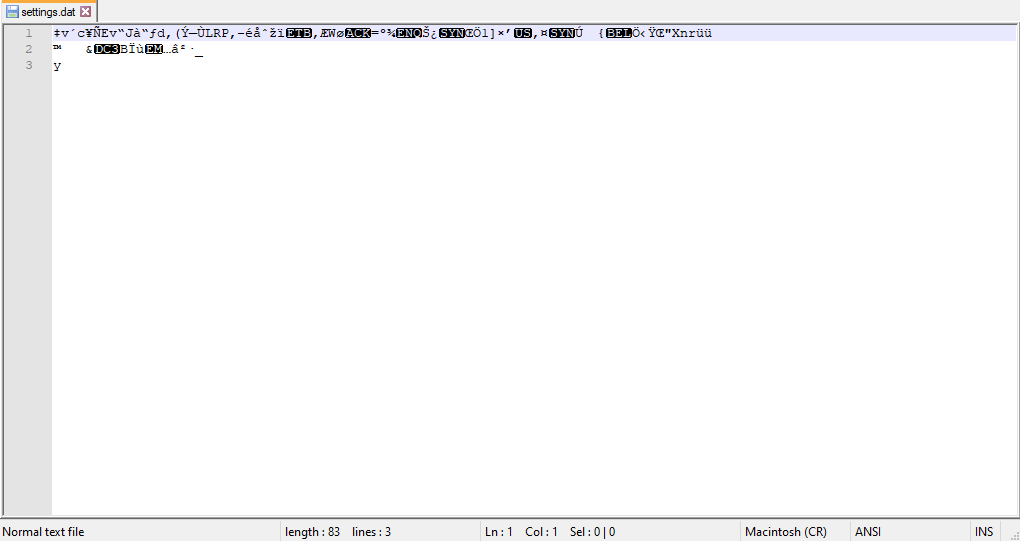
\includegraphics[width=1\textwidth, height=1\textheight, keepaspectratio]{./img/Applicativo/salvataggio_criptato.png}
	\caption{Salvataggio delle impostazioni e alert di conferma}
	\label{fig:encrypted_save_file}
\end{figure}

% ========================== QUIT TAB =========================================

\newpage

\subsection{Quit | Uscita}

\textsf{\small Infine, l'ultima sezione del software è l'uscita dal programma possibile sia dall'icone della crocetta rossa in alto a destra (che però non utilizza un Alert) sia dal menù \emph{Quit | Uscita} e dopo aver confermato l'uscita dall' \emph{Alert} si uscirà dal programma.}\\

\begin{figure}[H] 
	\centering
	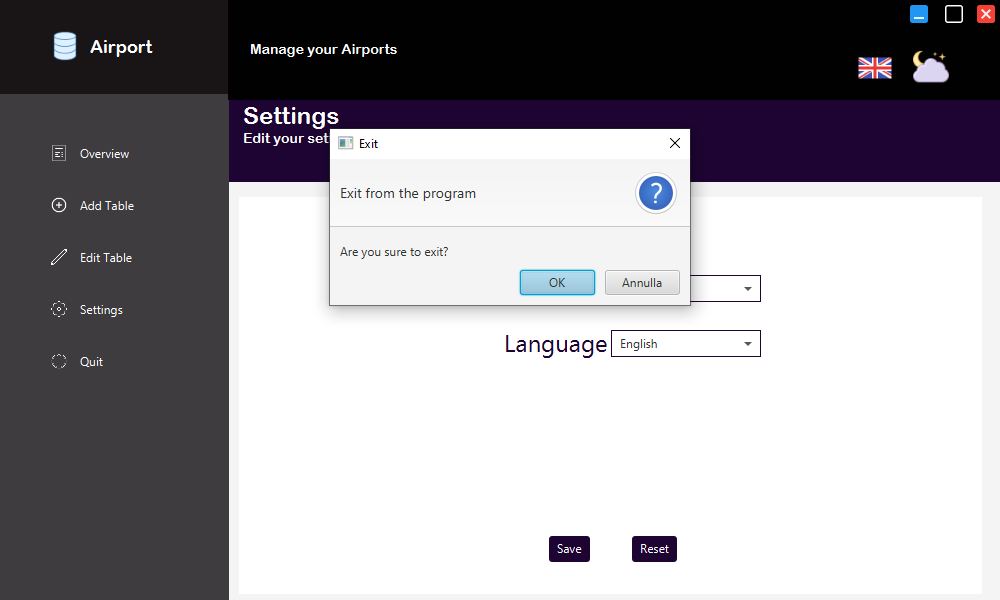
\includegraphics[width=1\textwidth, height=1\textheight, keepaspectratio]{./img/Applicativo/quit_alert.png}
	\caption{Alert di conferma per l'uscita}
	\label{fig:quit_alert}
\end{figure}